\section{Évaluation de l'hypothèse d'efficacité}
\label{section:4.1-HYPOTHESE-EFFICACITE}

	%%% Introduction / Transition.
	En premier lieu et afin de poser les bases de nos études, nous devons nous demander si notre implémentation du \textit{clustering} interactif est fonctionnel et si elle permet d'atteindre son objectif.
	Nous aimerions donc vérifier l'hypothèse suivante :
	
	%%% Formulation des hypothèses
	\begin{tcolorbox}[
		title=\faVial~\textbf{Hypothèse d'efficacité}~\faVial,
		colback=colorTcolorboxHypothesis!15,
		colframe=colorTcolorboxHypothesis!75,
		width=\linewidth
	]
		% Hypothèse.
		« \textbf{
			Une méthodologie d'annotation basée sur le \textit{clustering} interactif permet d'obtenir une base d'apprentissage pour un assistant conversationnel qui respecte la vision donnée par l'expert métier au cours de l'annotation.
		} » \\
		
		% Figure.
		La \textsc{Figure~\ref{figure:4.1-HYPOTHESE-EFFICACITE}} illustre cette hypothèse et l'espoir de convergence d'une base d'apprentissage en cours de construction vers sa vérité terrain.
		%
		\begin{figure}[H]  % keep [H] to be in the tcolorbox.
			\centering
			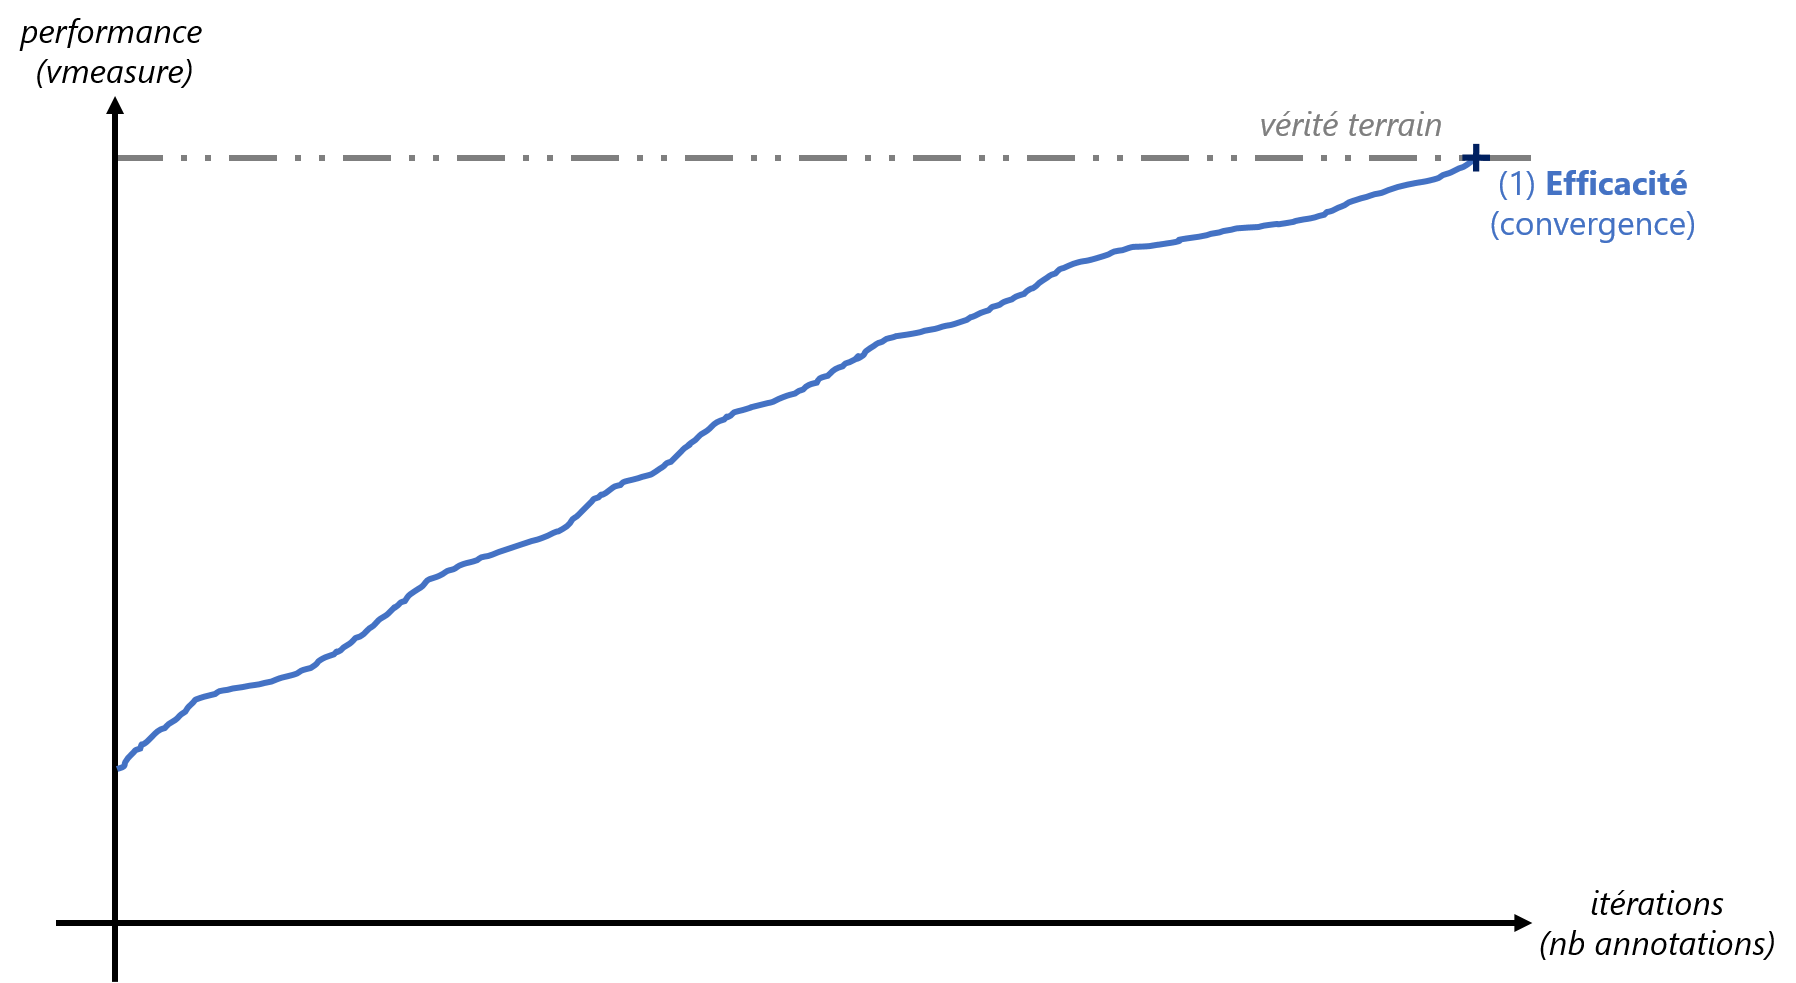
\includegraphics[width=0.95\textwidth]{figures/hypotheses-01-efficacite}
			\caption{
				Illustration des études réalisées sur le \textit{clustering} interactif (\textit{étape 1/6}) en schématisant l'évolution de la performance (\textit{accord avec la vérité terrain calculé en v-measure}) d'une base d'apprentissage en cours de construction en fonction du nombre d'itérations de la méthode (\textit{nombre d'annotations par un expert métier}).
			}
			\label{figure:4.1-HYPOTHESE-EFFICACITE}
		\end{figure}
	\end{tcolorbox}
		
	% Résumé de l'étude.
	Afin de vérifier cette hypothèse, nous mettons en place une \textbf{expérience de ré-annotation} d'une base d'apprentissage (qui servira ici de vérité terrain) à l'aide de notre méthode, en simulant l'annotation d'un expert, et nous critiquons l'évolution de la nouvelle base d'apprentissage obtenue ainsi que sa similitude avec la base d'apprentissage initiale (cf. \textsc{Section~\ref{section:4.1.1-ETUDE-CONVERGENCE}}).
	
	
	%%%
	%%% Subsection 4.1.1: Étude de convergence vers une vérité terrain pré-établie en simulant l'annotation d'une base d'apprentissage et mesurant la vitesse de sa création
	%%%
	\subsection{Étude de convergence vers une vérité terrain pré-établie en simulant l'annotation d'une base d'apprentissage et mesurant la vitesse de sa création}
	\label{section:4.1.1-ETUDE-CONVERGENCE}
		
		% Objectif de l'expérience.
		Nous voulons vérifier qu'une méthodologie d'annotation basée sur notre implémentation du \textit{clustering} interactif permet de créer une base d'apprentissage pour un assistant conversationnel.
		Pour cela, nous prenons une base d'apprentissage employée pour entraîner un modèle de classification de textes, et nous utilisons ce jeu de données comme vérité terrain.
		L'objectif de cette expérience est de simuler la création de cette base d'apprentissage et de nous assurer que le résultat obtenu correspond à la vérité terrain.
			
		% Référence articles.
		\begin{leftBarInformation}
			Cette étude a été l'objet d'une présentation à la conférence \texttt{EGC (Extraction et Gestion des Connaissances)}~(\cite{schild-etal:2021:conception-iterative-semisupervisee}), et d'une extension dans le journal \texttt{IJDWM (International Journal of Data Warehousing and Mining)}~(\cite{schild-etal:2022:iterative-semisupervised-design}).
			\footnote{Les résultats et la discussion de ces articles ont été mis à jour et réécrits pour mieux s'intégrer au discours ce manuscrit.}
		\end{leftBarInformation}

		%%% Protocole expérimental.
		\subsubsection{Protocole expérimental}
			
			% Axiome.
			\begin{leftBarWarning}
				Dans le cadre de cette étude, nous supposons que l'expert métier connaît parfaitement le domaine traité dans ce jeu de données, et qu'il est capable de caractériser sans ambiguïté la similitude entre deux données issues de cet ensemble.
				Cependant, cette hypothèse forte n'est pas toujours vérifiée en pratique, surtout lorsque l'on manipule des données non structurées.
				L'impact de ce point sur les résultats obtenus sera discuté en fin de partie, et nous nous y intéresserons plus en détails dans la \textsc{Section~\ref{section:4.6-HYPOTHESE-ROBUSTESSE}} (hypothèse de robustesse).
			\end{leftBarWarning}
			
			% Pseudo-code.
			Pour résumer le protocole expérimental que nous décrivons ci-dessous, vous pouvez vous référer au pseudo-code décrit dans \textsc{Algorithme~\ref{algorithm:4.1.1-ETUDE-CONVERGENCE-PROTOCOLE}}.
			
			\begin{algorithm}
				\KwData{jeu de données annoté (vérité terrain)}
				\KwIn{arrangements d'algorithmes et de paramètres à tester}
				%
				\ForEach{algorithmes et de paramètres à tester}{
					\textbf{initialisation (données)}: récupérer les données et la vérité terrain \;
					\textbf{initialisation (contraintes)}: créer une liste vide de contraintes \;
					\textbf{prétraitement}: supprimer le bruit dans les données \;
					\textbf{vectorisation}: transformer les données en vecteurs \;
					\textbf{clustering initial}: regrouper les données par similarité des vecteurs \;
					\textbf{évaluation}: estimer l'équivalence entre le \textit{clustering} obtenu et la vérité terrain \;
					\Repeat{annotation de toutes les contraintes possibles}{
						\textbf{échantillonnage}: sélectionner de nouvelles contraintes à annoter \;
						\textbf{simulation d'annotation}: caractériser les contraintes grâce à la vérité terrain \;
						\textbf{intégration}: ajouter les nouvelles contraintes au gestionnaire de contraintes \;
						\textbf{clustering}: regrouper les données par similarité avec les contraintes \;
						\textbf{évaluation}: estimer l'équivalence entre le \textit{clustering} obtenu et la vérité terrain \;
					}
					\textbf{évaluation finale}: espérer avoir un score d'équivalence de $100$\% avec la vérité terrain \;
				}
				%
				\KwResult{algorithmes et de paramètres ayant un score d'équivalence de $100$\%}
				%
				\caption{\textit{
					Description en pseudo-code du protocole expérimental de l'étude de convergence du \textit{clustering} interactif vers une vérité terrain pré-établie.
				}}
				\label{algorithm:4.1.1-ETUDE-CONVERGENCE-PROTOCOLE}
			\end{algorithm}
			
			% Description de la vérité terrain.
			Nous utilisons comme vérité terrain le jeu de données \texttt{Bank Cards (v1.0.0)} : ce dernier traite des demandes les plus fréquentes des clients en ce qui concerne la gestion de leur carte bancaire.
			Il est composé de $500$ questions rédigées en français et réparties en $10$ classes (\texttt{perte ou vol de carte}, \texttt{carte avalée}, \texttt{commande de carte}, ...).
			Pour plus de détails, consultez l'annexe~\ref{annex:C.1-DATASET-BANK-CARDS}.
			
			% Détails de l'expérience.
			Lors de cette expérience, chaque tentative de la méthode commencera sur la version non labellisée de la vérité terrain à disposition, sans aucune contrainte connue à l'avance.
			A chaque itération de la méthode, nous simulons l'annotation de l'expert métier en comparant les labels de la vérité terrain : ainsi, deux données ont une contrainte \texttt{MUST-LINK} si elles ont le même label, et une contrainte \texttt{CANNOT-LINK} sinon.
			Cela traduit le prérequis d'avoir un annotateur qui soit capable, dans son domaine d'expertise, de différencier deux données selon leur ressemblance.
			Une tentative de l'application de notre méthode s'arrête lorsque toutes les contraintes possibles entre les données ont été annotés par l'expert.

			% Description implémentation de l'interactive clustering.
			Pour cette étude, nous essayons une tentative pour chaque combinaison de paramètres de notre implémentation du \textit{clustering} interactif (cf. \textsc{Section~\ref{section:3.3-DESCRIPTION-IMPLEMENTATION}}). Cela comprend les tâches et leurs paramètres respectifs suivants :
			\begin{enumerate}
				\item le \textbf{prétraitement} des données, avec les niveaux suivants : \textbf{aucun} (noté \texttt{prep.no}), \textbf{simple} (noté \texttt{prep.simple}), avec \textbf{lemmatisation} (noté \texttt{prep.lemma}) et avec \textbf{filtres} (noté \texttt{prep.filter}) ;
				\item la \textbf{vectorisation} des données, avec les niveaux suivants : \textbf{TF-IDF} (noté \texttt{vect.tfidf}) et \textbf{SpaCy} (noté \texttt{vect.frcorenewsmd}) ;
				\item le \textbf{clustering sous contraintes} des données, avec les niveaux suivants : \textbf{KMeans} (modèle \textit{COP} noté \texttt{clust.kmeans.cop}), \textbf{Hiérarchique} (lien \textit{single} noté \texttt{clust.hier.sing} ; lien \textit{complete} noté \texttt{clust.hier.comp} ; lien \textit{average} noté \texttt{clust.hier.avg} ; lien \textit{ward} noté \texttt{clust.hier.ward}) et \textbf{Spectral} (modèle \textit{SPEC} noté \texttt{clust.spec}). Le choix du nombre de clusters n'est pas étudié ici, et ce nombre est fixé au nombre de classes présentes dans la vérité terrain ;
				\item l'\textbf{échantillonnage} des contraintes à annoter, avec les niveaux suivants : \textbf{purement aléatoire} (noté \texttt{samp.random.full}), \textbf{pseudo-aléatoire} (noté \texttt{samp.random.same}), \textbf{même cluster et étant les plus éloignées} (noté \texttt{samp.farhtest.same}) et \textbf{clusters différents et étant les plus proches} (noté \texttt{samp.closest.diff}). Le choix de la taille d'échantillon n'est pas étudié ici, et cette taille est arbitrairement fixée à $50$
				\footnote{Une taille d'échantillon de $50$ contraintes à annoter semble a priori un bon compromis entre (1) ne pas donner trop de travail à un annotateur en une session et (2) donner suffisamment de nouvelles contraintes au \textit{clustering} pour proposer un partitionnement plus pertinent des données. Ce choix sera discuté en fin de partie, et nous nous y intéresserons davantage dans la \textsc{Section~\ref{section:4.3-HYPOTHESE-COUTS}} (hypothèse sur les coûts).}.
			\end{enumerate}
			
			Il y a donc $192$ combinaisons testées, et chaque tentative est répétée $5$ fois pour contrer les aléas statistiques des algorithmes de \textit{clustering} (\textit{initialisation du \texttt{clust.kmeans.cop}, ...}) et d'échantillonnage (\textit{choix des contraintes au hasard avec \texttt{samp.random.full}, ...}).
			Pour plus de détails sur ces algorithmes, référez-vous à la \textsc{Section~\ref{section:3.3-DESCRIPTION-IMPLEMENTATION}} pour avoir accès à leur description, à leurs paramètres et aux choix d'implémentation.
			
			% Description de l'évaluation.
			Pour évaluer l'équivalence entre la vérité terrain et notre segmentation des données obtenue au cours de la méthode, nous nous intéressons à l'évolution de la \texttt{v-measure} (\cite{rosenberg-hirschberg:2007:vmeasure-conditional-entropybased}) entre ces deux jeu de données.
			Si le score du calcul de la \texttt{v-measure} est de $100$\%, cela signifierait que le \textit{clustering} final et la vérité terrain propose une segmentation identique des données, donc que la vérité terrain a pu être retrouvée, et donc qu'il est possible d'obtenir une base d'apprentissage pour un assistant conversationnel à l'aide d'une méthodologie d'annotation basée sur le \textit{clustering} interactif.
			
			% Référence scripts.
			\begin{leftBarInformation}
				Les scripts de l'expérience (\textit{notebooks} Python (\cite{van-rossum-drake:2009:python-reference-manual})) sont disponibles dans un dossier dédié de~\cite{schild:2021:cognitivefactory-interactiveclusteringcomparativestudy}.
			\end{leftBarInformation}

		%%% Résultats.
		\subsubsection{Résultats obtenus}
			
			% Graphe d'évolution de la v-measure moyenne, min et max.
			La \textsc{Figure~\ref{figure:4.1.1-ETUDE-CONVERGENCE-EVOLUTION}} et la \textsc{Table~\ref{table:4.1.1-ETUDE-CONVERGENCE-EVOLUTION}} représentent l'évolution moyenne de la \texttt{v-measure} du \textit{clustering} en fonction du nombre d'itération de la méthode. Les tentatives les plus rapides et les plus lentes sont représentées sur la figure.
							
			% Tendance: Forte dispersion, Croissance générale.
			Malgré une forte dispersion des résultats (écart-type de \texttt{v-measure} pouvant être supérieur à $20$\%, forte différence entre les tentatives la plus rapide et la plus lente) et quelques sauts de performances (cf. à-coups de la tentative la plus lente sur la figure), une convergence générale vers la vérité terrain peut être constatée.
			
			% Tendance à courts termes: Croissance linéaire
			A l'itération $0$, une tentative commence avec une moyenne de $19.05$\% de \texttt{v-measure}  entre son \textit{clustering} initial (sans contraintes) et la vérité terrain.
			Cette \texttt{v-measure} moyenne croît presque linéairement (pente de $0.97$) jusqu'à l'itération $75$ où elle atteint la performance de $92.08$\% (cf. \textsc{Table~\ref{table:4.1.1-ETUDE-CONVERGENCE-EVOLUTION}}).

			% Tendance à longs termes: Asymptote.
			Au delà de l'itération $75$, la courbe de la \texttt{v-measure} moyenne tend vers une asymptote de $100$\% (cf. \textsc{Figure~\ref{figure:4.1.1-ETUDE-CONVERGENCE-EVOLUTION}}).
			Cette asymptote est atteinte par toute les $960$ tentatives ($192$ combinaisons de paramètres, $5$ tentatives pour chaque combinaison), la tentative l'ayant atteinte le plus tôt à l'itération $19$ et celle le plus tard à l'itération $328$.
			
			% Tendances à terminer sans avoir toutes les contraintes.
			La courbe se prolonge jusqu'à l'itération $393$ pour que toutes les tentatives puisse annoter toutes les contraintes possibles sur le jeu de données.
			On peut aussi noter que $756$ tentatives ($78.75$\%) convergent vers $100$\% de \texttt{v-measure} avant l'annotation exhaustive de toutes les contraintes : sur ces tentatives, la convergence peut ainsi s'observer en moyenne avec seulement $91.30$\% du nombre de contraintes possibles (min: $8.72$\%, max: $99.69$\%, écart-type: $18.60$\%).
			
			%
			\begin{figure}[!htb]
				\centering
				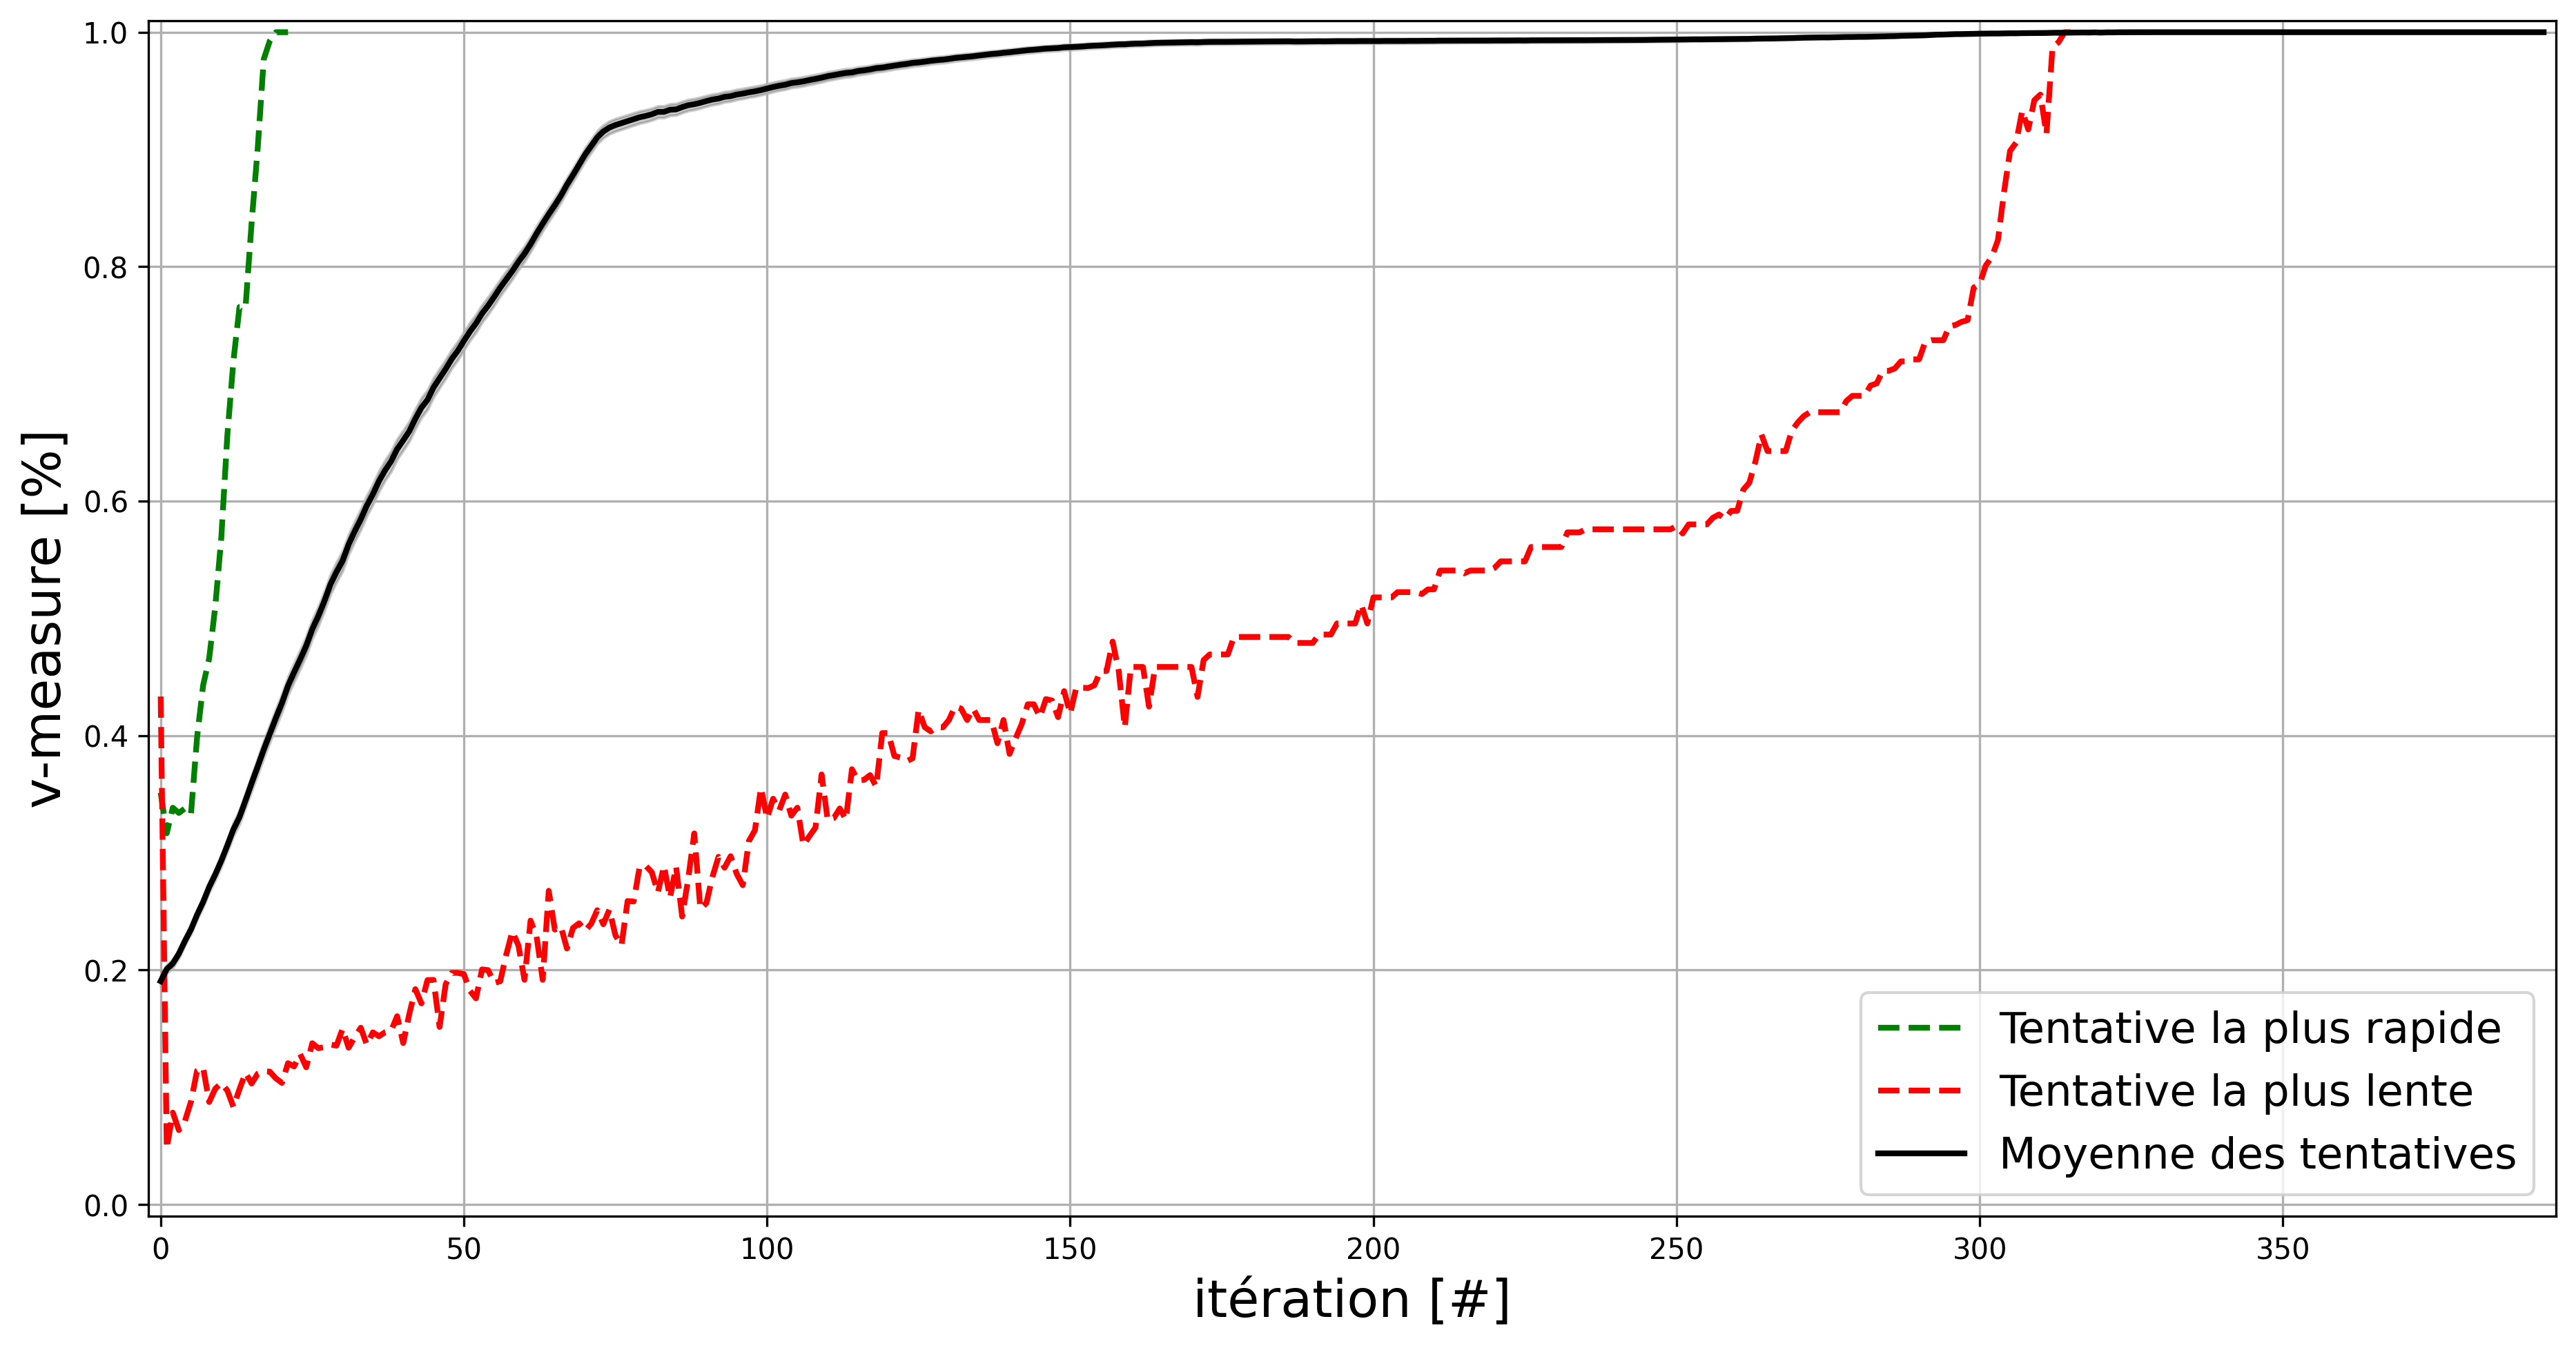
\includegraphics[width=0.95\textwidth]{figures/etude-efficacite-evolution-moyenne-0par-iteration}
				\caption{
					Évolution de la moyenne de la \texttt{v-measure} entre un résultat obtenu et la vérité terrain en fonction du nombre d'itération de la méthode de \textit{clustering} interactif, moyenne réalisée itération par itération sur l'ensemble des tentatives.
					Représentation des tentatives ayant été les plus rapides (\textit{un prétraitement \texttt{prep.simple}, une vectorisation \texttt{vect.tfidf}, un \textit{clustering} \texttt{clust.hier.comp} ou \texttt{clust.hier.ward}, et un échantillonnage \texttt{samp.closest.diff}}) et les plus lentes (\textit{un prétraitement \texttt{prep.no}, une vectorisation \texttt{vect.tfidf}, un \textit{clustering} \texttt{clust.spec}, et un échantillonnage de contraintes \texttt{samp.farthest.same}}) pour atteindre $100$\% de \texttt{v-measure}.
				}
				\label{figure:4.1.1-ETUDE-CONVERGENCE-EVOLUTION}
			\end{figure}
			%
			\begin{table}[!htb]
				\begin{center}
				\begin{tabular}{|c|r|r|r|r|r|}
					\hline
					% ENTETE DU TABLEAU
					\multicolumn{2}{|c|}{ \shortstack{ Annotations } }
						& \multicolumn{4}{c|}{ \shortstack{ Performances (\texttt{v-measure}) } }
						\tabularnewline
						\hline
					\multicolumn{1}{|c|}{ \shortstack{ Itérations } }
						& \multicolumn{1}{c|}{ \shortstack{ Contraintes } }
						& \multicolumn{1}{c|}{ \shortstack{ Moyenne } }
						& \multicolumn{1}{c|}{ \shortstack{ Écart-type } }
						& \multicolumn{1}{c|}{ \shortstack{ Minimum } }
						& \multicolumn{1}{c|}{ \shortstack{ Maximum } }
						\tabularnewline
						\hline
					%
					$0$		& $0$		& $19.05$\% \footnotesize $(\pm0.43)$ \par	& $13.38$\% & $03.42$\% & $47.75$\%
					\tabularnewline
					\hline
					%
					$25$	& $1~250$	& $49.09$\% \footnotesize $(\pm0.82)$ \par	& $25.43$\% & $09.09$\% & $100.00$\%
					\tabularnewline
					\hline
					%
					$50$	& $2~500$	& $73.66$\% \footnotesize $(\pm0.77)$ \par	& $23.98$\% & $16.78$\% & $100.00$\%
					\tabularnewline
					\hline
					%
					$75$	& $3~750$	& $92.08$\% \footnotesize $(\pm0.54)$ \par	& $16.70$\% & $21.74$\% & $100.00$\%
					\tabularnewline
					\hline
					%
					$100$	& $5~000$	& $95.19$\% \footnotesize $(\pm0.41)$ \par	& $12.67$\% & $26.93$\% & $100.00$\%
					\tabularnewline
					\hline
					%
					$125$	& $6~250$	& $97.43$\% \footnotesize $(\pm0.29)$ \par	& $09.09$\% & $34.99$\% & $100.00$\%
					\tabularnewline
					\hline
					%
					$150$	& $7~500$	& $98.73$\% \footnotesize $(\pm0.23)$ \par	& $07.22$\% & $38.14$\% & $100.00$\%
					\tabularnewline
					\hline
					%
					$328$	& $16~400$	& $100.00$\% \footnotesize $(\pm0.00)$ \par	& $0.00$\% & $100.00$\% & $100.00$\%
					\tabularnewline
					\hline
					%
					$394$	& $19~700$	& $100.00$\% \footnotesize $(\pm0.00)$ \par	& $0.00$\% & $100.00$\% & $100.00$\%
					\tabularnewline
					\hline
					
				\end{tabular}
				\end{center}
				\caption{
					Détails de l'évolution de la moyenne de la \texttt{v-measure} entre un résultat obtenu et la vérité terrain en fonction du nombre d'itération de la méthode de \textit{clustering} interactif, moyenne réalisée itération par itération sur l'ensemble des tentatives.
				}
				\label{table:4.1.1-ETUDE-CONVERGENCE-EVOLUTION}
			\end{table}

		%%% Discussion.
		\subsubsection{Discussion}
			
			%%% Avantages : il y a convergence !
			Au regard des résultats décrits ci-dessus, les différentes simulations de la méthode ont bien convergé vers la vérité terrain (atteinte de l'asymptote à $100$\% de \texttt{v-measure}).
			Cette expérience permet donc de confirmer plusieurs espoirs portés sur la méthode.
			
			% Avantage 1 : Émergence d'une modélisation sur la base des contraintes
			Tout d'abord, la vérité terrain a été retrouvée sans formaliser concrètement la structure de données.
			Là où une annotation par label aurait requis au préalable une définition des catégories possibles pour les données à étiqueter (création d'un "\textit{type system}"), la méthodologie employant le \textit{clustering} interactif a permis de faire émerger naturellement cette structure de données.
			Cette émergence provient directement des contraintes annotées par l'expert métier, traduisant ainsi ses connaissances à l'aide d'instructions simples : \textit{les données sont-elles ou non similaires ?}
			Cela représente un net avantage pour l'opérateur qui n'a ainsi pas à maintenir en mémoire une modélisation complexe de la structure de données, rendant la tâche d'annotation plus accessible.
			
			% Avantage 2 : Annotations plus simples et plus concrètes
			D'autre part, ces contraintes ont été l'objet d'une annotation guidée par les besoins de la machine afin de s'améliorer d'itération en itération (voir la croissance globale de la \texttt{v-measure} sur la \textsc{Figure~\ref{figure:4.1.1-ETUDE-CONVERGENCE-EVOLUTION}}).
			Ainsi, l'expert métier corrige la base d'apprentissage à chaque itération : soit en affinant les clusters en cours de construction, améliorant ainsi la cohérence des clusters (cf. pentes croissantes) ; soit en remaniant les clusters mal formés pour repartir sur de bonnes bases, détériorant la cohérence des clusters le temps de la réorganisation (cf. oscillations ou pentes décroissantes).
			Une telle assistance limite ainsi le nombre de contraintes non utiles au \textit{clustering}, même si certains paramétrages semblent plus efficaces que d'autres (voir la forte dispersion des résultats).
			
			% Avantage 3 : Pas besoins d'une exhaustivité de contraintes.
			De plus, nous remarquons que $76.75$\% des tentatives convergent vers la vérité terrain sans bénéficier d'une annotation exhaustive de toutes les contraintes possibles.
			Cela montre l'intérêt des interactions homme/machine afin d'obtenir plus efficacement un résultat qu'un expert métier (aussi parfait soit-il) aurait obtenu seul. 
			L'intérêt serait maintenant de déterminer la meilleure combinaison de paramétrage demandant d'annoter un nombre \textbf{suffisant} de contraintes afin d'obtenir ce même résultat de la manière la plus efficiente (cf. \textsc{Section~\ref{section:4.2-HYPOTHESE-EFFICIENCE}}) et la plus robuste aux erreurs d'annotation (cf. \textsc{Section~\ref{section:4.6-HYPOTHESE-ROBUSTESSE}}).
			\\

			
			%%% Limites.
			Néanmoins, différentes pistes sont encore à explorer pour rendre le \textit{clustering} interactif utilisable en situation réelle.
			
			% Limite 1 : Nombre d'annotations ==> besoin d'optimisation.
			D'une part, nous échangeons le besoin de définir une structure de données contre la nécessité d'annoter un grand nombre de contraintes : pour $500$ points de données, et en considérant que l'asymptote à $100$\% est atteinte en moyenne autour de l'itération $200$, il faudrait $10~000$ annotations de contraintes pour être exhaustif, ce qui correspond à près de $20$ fois plus de contraintes que de données.
			Bien que l'annotation binaire demande a priori une charge mentale plus faible (\cite{hart-staveland:1988:development-nasatlx-task}) et que l'opérateur n'a pas besoin de définir ou de maintenir en mémoire une structure de données complexe, un tel volume d'annotation représente tout de même une grande quantité de travail.
			Cela peut décourager les experts métiers en début de projet, surtout pour des projets ayant des jeux de données de plus grandes tailles.
			Toutefois, les résultats obtenus montrent une forte dispersion du nombre d'itérations nécessaire, et certaines tentatives ont été bien plus efficientes dans l'utilisation de leurs contraintes. La tentative la plus rapide a convergé à l'itération $19$, soit $950$ contraintes, ce qui est un volume d'annotation bien plus abordable !
			On peut donc espérer trouver un paramétrage optimal de la méthode permettant de diminuer significativement le nombre moyen de contraintes nécessaires afin d'obtenir une base d'apprentissage exploitable avec un volume d'annotations acceptable.
			Cet aspect fait l'objet de l'étude décrite dans la \textsc{Section~\ref{section:4.2-HYPOTHESE-EFFICIENCE}} (hypothèse d'efficience).
			
			% Limite 2 : Exhaustivité des annotations ==> evaluation de la rentabilité.
			D'autre part, le choix d'annoter toutes les contraintes possibles sur les données (\textbf{annotation exhaustive}) n'est pas forcément judicieux.
			En effet, si nous nous regardons la \textsc{Figure~\ref{figure:4.1.1-ETUDE-CONVERGENCE-EVOLUTION}}, une moyenne de $90$\% de \texttt{v-measure} est déjà atteinte autour de l'itération $75$, alors que l'asymptote à $100$\% n'est atteinte qu'au delà de l'itération $200$.
			Afin d'être plus efficient, il faudrait envisager une \textbf{annotation partielle} permettant d'obtenir rapidement ces $90$\% de \texttt{v-measure} (cf. coude sur la \textsc{Figure~\ref{figure:4.1.1-ETUDE-CONVERGENCE-EVOLUTION}}), quitte à affiner le résultat manuellement pour combler la "perte" moyenne de $10$\% de \texttt{v-measure}.
			Cet aspect sera ajouté à l'objectif de l'étude décrite dans la \textsc{Section~\ref{section:4.2-HYPOTHESE-EFFICIENCE}} (hypothèse d'efficience).
			
			% Limite 3 : Expert métier parfait ==> simuler les erreurs.
			Pour finir, nous avons supposé dans cette étude que l'annotateur est un expert métier connaissant parfaitement le domaine traité.
			Cette hypothèse forte n'est a priori pas valable en situation réelle : En effet, des erreurs d'annotations peuvent intervenir (ambiguïtés sur les données, méconnaissance du domaine, erreurs d'inattention, différence d'opinions entre annotateurs, ...), ce qui peut entraîner des divergences ou des incohérences dans la construction de la base d'apprentissage.
			Il semble donc nécessaire d'étudier les impacts de ces incohérences, ainsi que de proposer une méthode pour les prévenir ou les corriger.
			Cet aspect sera traité à la fin de ce chapitre dans la \textsc{Section~\ref{section:4.6-HYPOTHESE-ROBUSTESSE}} (hypothèse de robustesse).